\documentclass[11pt,a4paper]{article}
\usepackage[a4paper,margin=2.3cm]{geometry}
\usepackage{amsmath,amssymb,mathtools}
\usepackage{fontspec}
\usepackage{polyglossia}
\setmainlanguage{russian}
\setotherlanguage{english}
\setmainfont{Liberation Serif}
\setsansfont{Liberation Sans}
\setmonofont{Liberation Mono}
\newfontfamily\cyrillicfont[Ligatures=TeX]{Liberation Serif}
\newfontfamily\cyrillicfontsf[Ligatures=TeX]{Liberation Sans}
\newfontfamily\cyrillicfonttt{Liberation Mono}
\usepackage{booktabs}
\usepackage{array}
\usepackage{enumitem}
\usepackage{graphicx}
\usepackage{float}
\usepackage{xcolor}
\usepackage[hidelinks]{hyperref}

\setlength{\parindent}{0pt}
\setlength{\parskip}{0.55em}
\emergencystretch=3em
\setlist{itemsep=0.25em,topsep=0.3em}

\newcommand{\norm}[1]{\lVert #1\rVert_2}
\newcommand{\E}{\mathbb{E}}
\DeclareMathOperator{\diag}{diag}
\DeclareMathOperator{\sigm}{sigm}
\DeclareMathOperator{\Var}{Var}
\makeatletter\newcommand{\tabinput}[1]{\@@input #1 }\makeatother
\renewcommand{\figurename}{Рис.}

\title{Раздел 3: обязательные численные эксперименты\\[0.2em]
\large логистическая регрессия и двухслойная сеть, SGD против R-SGD}
\author{Homework Mini-Project: SGD versus Robust SGD under Gradient Uncertainty}
\date{17 ноября 2026 г.}

\begin{document}
\maketitle

\section*{Постановка и краткие результаты}

Раздел 3 требует двух экспериментов: однослойной логистической регрессии на гауссовских
кластерах и двухслойной $\tanh$-сети на зашумлённых полуокружностях. В каждом SGD и R-SGD
сравниваются при неопределённости градиента, с оценкой на чистых данных, как минимум при
одном уровне без искусственного шума и одном зашумлённом. Для каждого эксперимента нужны:
кривые потерь на обучающей и валидационной выборках при всех уровнях шума; итоговые
потери на обучении, потери на тесте, точность, время работы и доля нулевых шагов; граница
решения для указанного сида оценки; обсуждение того, совпадают ли ранжирования по
оптимизации и по предсказанию. Честное сравнение требует также протокола настройки и
оценки из раздела 4, поэтому его пункты 1--4 реализованы здесь же.

Основные выводы. Это эмпирические результаты для двух данных задач и данных настроек, а не
общие утверждения.
\begin{itemize}
\item \textbf{Логистическая регрессия.} Оба метода достигают байесовской точности ($0.922$
против $0.923$ у байесовского правила на тех же тестовых выборках) при всех уровнях шума,
кроме наибольшего. R-SGD немного снижает потери на обучении при $c=0,1$ (на
$0.001$--$0.003$, устойчиво на фиксированном наборе данных: 10/10 и 9/10 сидов), но
точность не меняется. С настройками, зафиксированными при $c=1$, R-SGD хуже SGD при $c=4$ и
заметно хуже при $c=16$.
\item \textbf{Двухслойная сеть.} Без искусственного шума R-SGD достигает гораздо меньших
потерь на обучении ($0.0019$ против $0.0110$, 10/10 сидов) и меньших потерь на тесте (9/10),
но не более высокой точности (3 победы, 2 ничьи). SGD с той же средней длиной шага не хуже
(R-SGD лучше в 4/10). При $c\ge1$ зафиксированная настройка R-SGD хуже SGD по потерям на тесте
и по точности, а при $c=16$ разваливается в 8 из 10 сидов (итоговые потери выше начальных
$\log2$).
\item \textbf{Почему.} Когда добавленный шум доминирует, $S_k\approx sI$, и робастный шаг
сводится к SGD с длиной шага, умноженной примерно на $(1-\rho/\sqrt p)$. Измеренные отношения
шагов $0.744$, $0.505$, $0.269$ при $\rho/\sqrt p=0.25,0.5,0.75$. Такой шаг не убирает шум, а
только укорачивает шаг, причём большие (шумные) градиенты он сжимает относительно
\emph{слабее}. Везде, где R-SGD улучшил потери при переборе радиуса, SGD с той же длиной шага
дал то же или лучше, с одним исключением: при малом шуме в логистической регрессии
сжатие R-SGD, зависящее от отношения сигнал/шум, выигрывало у постоянного уменьшения шага по
потерям (5/5 сидов при каждом радиусе) — как адаптивное расписание, — но опять без изменения
точности.
\item \textbf{Нулевые шаги до минимума.} В сети радиусы $\rho\gtrsim\sqrt p$ дают 35--100\%
нулевых шагов и останавливают обучение далеко от любого минимума (точность на тесте
$0.86$--$0.50$); при шуме и $\rho=2\sqrt p$ сеть вообще не уходит от начальной точки.
\item \textbf{Оптимизация и предсказание.} При малом шуме ранжирование по потерям на
обучении совпадает с ранжированием по потерям на тесте, но не по точности (совпадение в
$2$--$5$ из 10 сидов). При большом шуме все три ранжирования совпадают (SGD лучше).
\end{itemize}

\section*{Шаг 1. Общий протокол}

\begin{center}
\small
\begin{tabular}{@{}p{0.27\linewidth}p{0.68\linewidth}@{}}
\toprule
Элемент & Выбор и причина \\
\midrule
Данные & сбалансированные классы; $n_{\rm train}=400$, $n_{\rm val}=400$, $n_{\rm test}=4000$,
выбираются независимо (большая тестовая выборка: стандартная ошибка точности $\le0.005$) \\
Предобработка & стандартизация $a\mapsto(a-\bar a_{\rm train})/s_{\rm train}$ по среднему и
стандартному отклонению \emph{только обучающей} выборки, применяется ко всем трём выборкам \\
Потери & $\ell(t,y)=\log(1+e^t)-yt$, вычисляются как \texttt{logaddexp(0,t)-y*t}; цель —
средние потери на обучении без регуляризатора; класс $=\mathbf 1[t>0]$ \\
Батч и бюджет & $b=16$, выбор с возвращением; $K=500$ обновлений (логистическая), $K=3000$
(сеть); $bK$ вычислений градиента за запуск у обоих методов \\
Шаги & $\alpha_k=\alpha_0/\sqrt{1+k/50}$ для обоих методов \\
Шум градиента & $v_{k,i}=u_i(\theta_k)+\sigma z_{k,i}$, $z_{k,i}\sim\mathcal N(0,I_p)$, независимы
по наблюдениям и итерациям; $\sigma=c\,\gamma$, $c\in\{0,1,4,16\}$ \\
Единица шума $\gamma$ & среднеквадратичное значение чистых градиентов примеров в начальной
точке, усреднённое по сидам настройки: $\gamma=0.500$ (логистическая), $\gamma=0.215$ (сеть) \\
Модель неопределённости & $g_k$, $S_k$ по формуле (4) из \emph{тех же} $b$ наблюдений, что
используются в обновлении \\
Оценка & все потери и точности на чистых данных; 61 контрольная точка на запуск для кривых \\
\bottomrule
\end{tabular}
\end{center}

\textbf{Уровни шума.} $c=0$ — случай без искусственного искажения (только шум выбора
мини-батча). При $c=1$ искажение одного наблюдения сравнимо с типичной координатой градиента
примера. При $c=4$ и $c=16$ оно доминирует. После усреднения по $b=16$ наблюдениям добавленный
шум в $g_k$ имеет стандартное отклонение $c\gamma/4$ на координату.

\textbf{Масштаб радиуса.} Радиус параметризуется как $\rho=r\sqrt p$. Вблизи стационарной
точки $g_k^TS_k^{-1}g_k$ приближённо распределено как $\chi^2_p$ со средним $p(b-1)/(b-3)$
(раздел 2, шаг 5), поэтому порог правила нулевого шага растёт как $\sqrt p$. Фиксированное
$\rho$ означало бы совсем разное при $p=3$ и $p=33$; в терминах $r$ смысл одинаков: $r\approx1$
— точка, с которой вблизи минимума начинаются нулевые шаги.

\textbf{Настройка (раздел 4.2).}
\begin{itemize}
\item Сетки: $\alpha_0\in\{0.1,0.3,1,3,10,30\}$ для обоих методов; $r\in\{0,0.25,0.5,0.75,1,1.25\}$
для R-SGD. $r=0$ включено, и R-SGD с $r=0$ — это SGD.
\item Данные для настройки: 3 сида настройки со своими наборами данных, инициализациями, батчами и
шумом, не пересекающиеся с сидами оценки; уровень шума при настройке $c=1$. Тестовые данные не
используются.
\item Критерий: среднее по сидам настройки значение потерь на валидации, усреднённых по последним
5 из 61 контрольной точки. Запуск считается неудачным, если потери на обучении становятся
бесконечными или превышают начальные в 50 раз.
\item Бюджеты поиска: SGD $6\times3=18$ запусков, R-SGD $36\times3=108$ запусков. Больший бюджет
даёт R-SGD преимущество (это минимум по большему числу шумных оценок); это обсуждается ниже.
\item После настройки параметры фиксируются и без изменений используются на всех уровнях шума.
\end{itemize}

\textbf{Оценка (раздел 4.3).} Две схемы по 10 сидов, парные по методам (одни и те же данные,
инициализация, индексы батчей и реализации шума $z_{k,i}$):
\begin{itemize}
\item \textbf{A} (меняется набор данных): каждый сид генерирует новые обучающую, валидационную и
тестовую выборки, новую инициализацию, новые батчи и новый шум. Разброс в A объединяет
неопределённость по наборам данных и случайность обучения.
\item \textbf{B} (только случайность обучения): набор данных A-сида 0 зафиксирован; меняются
инициализация, батчи и шум.
\end{itemize}
Погрешности: «среднее $\pm$ sd» — среднее и выборочное стандартное отклонение по 10 сидам
(разброс результатов). Для парных разностей «среднее $\pm$ h» даёт полуширину $h$
95\%-го $t$-интервала для средней разности, «победы» — число сидов, где R-SGD лучше (ничьи в
скобках).

\textbf{Дополнения (раздел 4.4).} (i) Перебор радиуса $r\in\{0,\dots,2\}$ при настроенном
$\alpha_0$ для SGD, 5 сидов. (ii) Контроль длины шага: SGD с
$\alpha_0'=\alpha_0\cdot\overline{\|d_k\|/(\alpha_k\|g_k\|)}$, средним отношением шагов
соответствующих запусков R-SGD (нулевые шаги дают 0). Он запускается для зафиксированной
настройки и для каждой точки перебора на тех же сидах.

\section*{Шаг 2. Эксперимент 1: логистическая регрессия}

\subsection*{2.1 Модель, градиент и эталон}

$a\mid y\sim\mathcal N\big((2y-1)(1,1)^T,I_2\big)$, $t_\theta(a)=w^Ta+c$, $\theta=(w_1,w_2,c)$,
$p=3$, $\theta_0=0$ (задача выпукла, поэтому фиксированная начальная точка естественна).
Градиент примера $u_i(\theta)=(\sigm(t_i)-y_i)\,(a_i^T,1)^T$ (раздел 2, шаг 3). Проверка
конечными разностями на данных оценки даёт относительные ошибки $2.7\cdot10^{-10}$ (средний
градиент) и $1.9\cdot10^{-10}$ (по примерам).

\textbf{Эталон.} Модель корректно специфицирована: логарифм отношения правдоподобий
$\log\frac{p(a\mid1)}{p(a\mid0)}=2\,(1,1)a$, поэтому байесовское правило — $a_1+a_2>0$ с
точностью $\Phi(\sqrt2)\approx0.921$. На фактических тестовых выборках схемы A байесовское
правило имеет точность $0.9228\pm0.0031$ и потери $0.1905\pm0.0065$ (истинный логит
$2(a_1+a_2)$). В среднем ни один метод не может быть лучше.

\subsection*{2.2 Настройка}

\begin{figure}[H]
\centering
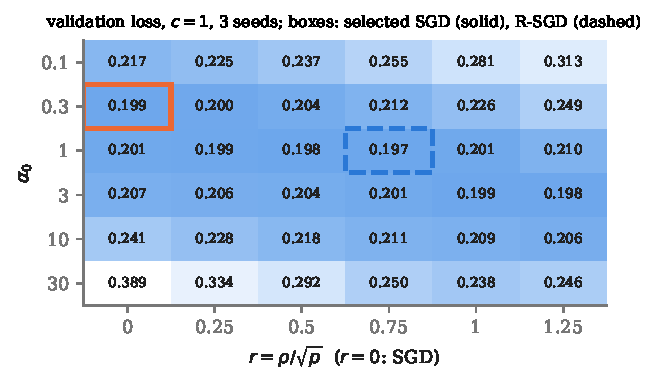
\includegraphics[width=0.49\linewidth]{../fig3/logreg_tuning.pdf}\hfill
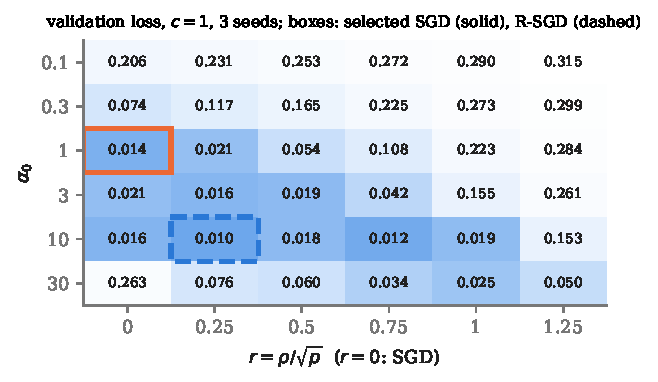
\includegraphics[width=0.49\linewidth]{../fig3/mlp_tuning.pdf}
\caption{Критерий настройки (средние потери на валидации, $c=1$, 3 сида настройки) для
логистической регрессии (слева) и сети (справа). Столбец $r=0$ — SGD. Рамки отмечают
выбранные настройки. (Подписи на рисунках на английском.)}
\label{fig:tuning}
\end{figure}

Выбрано: SGD $\alpha_0=0.3$; R-SGD $\alpha_0=1$, $r=0.75$ ($\rho=1.30$). Ни одна настройка не
лежит на краю сетки. Критерий очень плоский: 10 из 36 клеток отличаются от лучшей ($0.197$) не
более чем на $0.005$. Область малых значений идёт по диагонали: больший $\alpha_0$ компенсируется
большим $r$, например $(1,0.75)$, $(3,1)$, $(3,1.25)$ почти равны. Это и есть взаимодействие шага
обучения и радиуса, о котором спрашивает раздел 5(b): оба управляют эффективной длиной шага.

\subsection*{2.3 Результаты}

\begin{figure}[H]
\centering
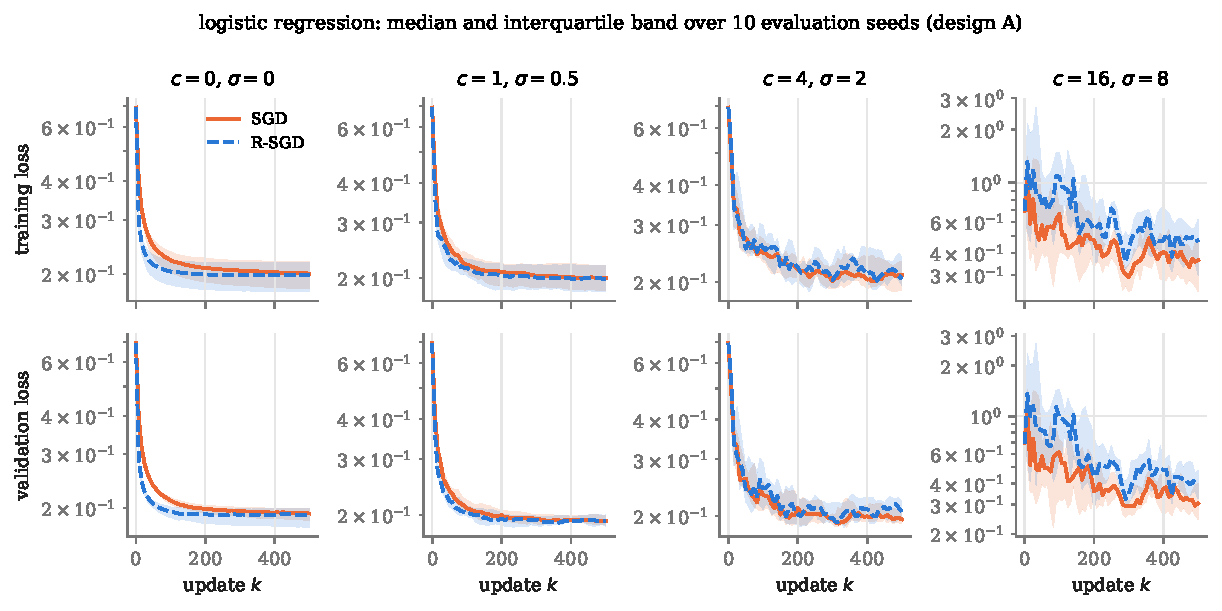
\includegraphics[width=\linewidth]{../fig3/logreg_curves.pdf}
\caption{Логистическая регрессия: потери на обучении (сверху) и на валидации (снизу) на чистых
данных в зависимости от номера обновления; медиана и интерквартильная полоса по 10 сидам оценки
(схема A). Зафиксированные настройки: SGD $\alpha_0=0.3$; R-SGD $\alpha_0=1$, $\rho=1.30$.}
\label{fig:lr_curves}
\end{figure}

\begin{center}
\small
\setlength{\tabcolsep}{4pt}
\begin{tabular}{@{}clccccc@{}}
\toprule
$c$ & метод & \shortstack{итог.\ потери\\обуч.} & \shortstack{потери\\на тесте} & \shortstack{точность\\на тесте} & \shortstack{нулевые\\шаги} & \shortstack{время, мс\\(мкс/обн.)} \\
\midrule
\tabinput{../tabs3/tab_lr_main.tex}
\bottomrule
\end{tabular}

\smallskip
Логистическая регрессия, схема A, среднее $\pm$ sd по 10 сидам; $bK=8000$ вычислений градиента
за запуск у обоих методов; байесовское правило: точность $0.9228$, потери на тесте $0.1905$.
\end{center}

\begin{center}
\footnotesize
\setlength{\tabcolsep}{2.6pt}
\begin{tabular}{@{}cccccccccc@{}}
\toprule
& & \multicolumn{2}{c}{$\Delta$ потерь обуч.} & \multicolumn{2}{c}{$\Delta$ потерь на тесте}
& \multicolumn{2}{c}{$\Delta$ точности} & \multicolumn{2}{c}{совпадение} \\
\cmidrule(lr){3-4}\cmidrule(lr){5-6}\cmidrule(lr){7-8}\cmidrule(lr){9-10}
$c$ & схема & среднее $\pm$ h & побед & среднее $\pm$ h & побед & среднее $\pm$ h & \shortstack{побед\\(ничьи)} & \shortstack{об.$\to$\\тест} & \shortstack{об.$\to$\\точн.} \\
\midrule
\tabinput{../tabs3/tab_lr_paired.tex}
\bottomrule
\end{tabular}

\smallskip
Парные разности R-SGD $-$ SGD (отрицательная разность потерь и положительная разность точности
в пользу R-SGD); «совпадение ранжирования» — число сидов, в которых знак $\Delta$ потерь на
обучении предсказывает знак $\Delta$ потерь на тесте (об.$\to$тест) или $-\Delta$ точности
(об.$\to$точн.).
\end{center}

Как читать результаты.
\begin{itemize}
\item \textbf{Точность насыщена.} При $c\le4$ оба метода отстоят от байесовской точности не
более чем на $0.005$, а средняя разность точностей по модулю меньше $0.001$. Разности потерь в
несколько тысячных сдвигают линейную границу пренебрежимо мало (рис.~\ref{fig:lr_bound}).
\item \textbf{Малый, но устойчивый выигрыш по потерям при $c\le1$.} На фиксированном наборе
данных (схема B) у R-SGD меньше потери на обучении в 10/10 ($c=0$) и 9/10 ($c=1$) сидов и
меньше потери на тесте в 10/10 и 8/10. При смене наборов данных (схема A) те же разности
скрываются гораздо большим разбросом между наборами (sd потерь на тесте $0.007$ в A против
$0.001$ в B при $c=0$).
\item \textbf{Хуже при $c\ge4$ с зафиксированными настройками.} R-SGD работает с
$\alpha_0=1$, втрое большим, чем у SGD, и полагается на сжатие как на компенсацию. Когда шум
доминирует, сжатие почти постоянно (шаг 4), большие шумные градиенты проходят, и потери выше:
$+0.005$ при $c=4$ и $+0.095$ при $c=16$; SGD лучше в 7--8 из 10 сидов.
\item \textbf{Нулевые шаги:} 18\% обновлений при $c=0$ и 32--33\% при $c\ge1$, включая
обновления в начале обучения. Они не помешали сходимости, поскольку $p=3$, а остальные шаги
большие.
\item \textbf{Время:} SGD 16--21\,мкс на обновление, R-SGD 58--88\,мкс (в 2.8--4.4 раза больше)
при одинаковом числе вычислений градиента.
\end{itemize}

\begin{figure}[H]
\centering
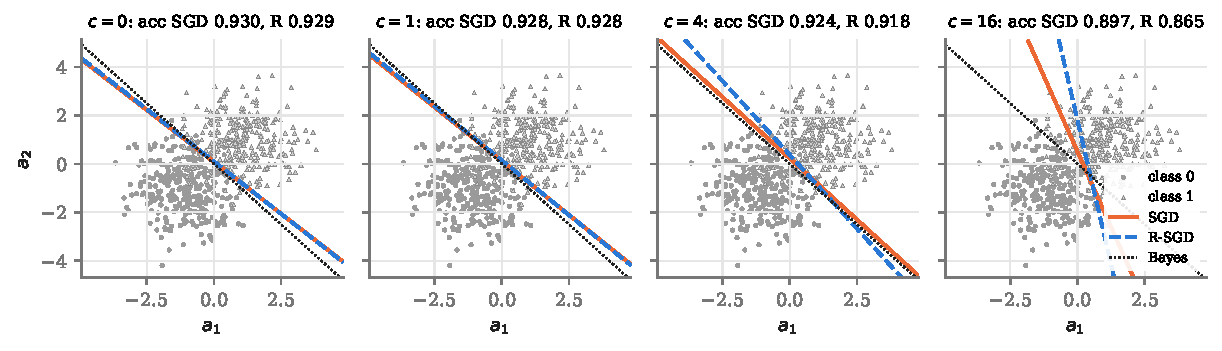
\includegraphics[width=\linewidth]{../fig3/logreg_boundaries.pdf}
\caption{Логистическая регрессия, сид оценки A-0 (сид данных указан в шаге 6): границы решения
$t_\theta(a)=0$ итоговых точек SGD и R-SGD в исходных координатах, байесовская граница
$a_1+a_2=0$ и 600 тестовых точек.}
\label{fig:lr_bound}
\end{figure}

\subsection*{2.4 Длина шага, чувствительность и разброс}

\begin{center}
\small
\setlength{\tabcolsep}{4pt}
\begin{tabular}{@{}cccccccc@{}}
\toprule
$c$ & \shortstack{отн.\\шага} & $\alpha_0'$ & потери R-SGD & \shortstack{потери SGD\\с той же длиной} & $\Delta$ (R $-$ контр.) & побед & \shortstack{точн.\\R / контр.} \\
\midrule
\tabinput{../tabs3/tab_lr_matched.tex}
\bottomrule
\end{tabular}

\smallskip
Зафиксированный R-SGD против SGD с той же средней длиной шага, схема A, 10 сидов (потери на
тесте).
\end{center}

При $c=0$ подобранный шаг в точности равен настроенному для SGD значению $0.3$, и методы равны
(5/10). При $c=1$ R-SGD выигрывает у контроля в 9/10 сидов на $0.003$ по потерям на тесте. При
$c\ge4$ контрольный SGD лучше, при $c=16$ — на $0.14$.

\begin{figure}[H]
\centering
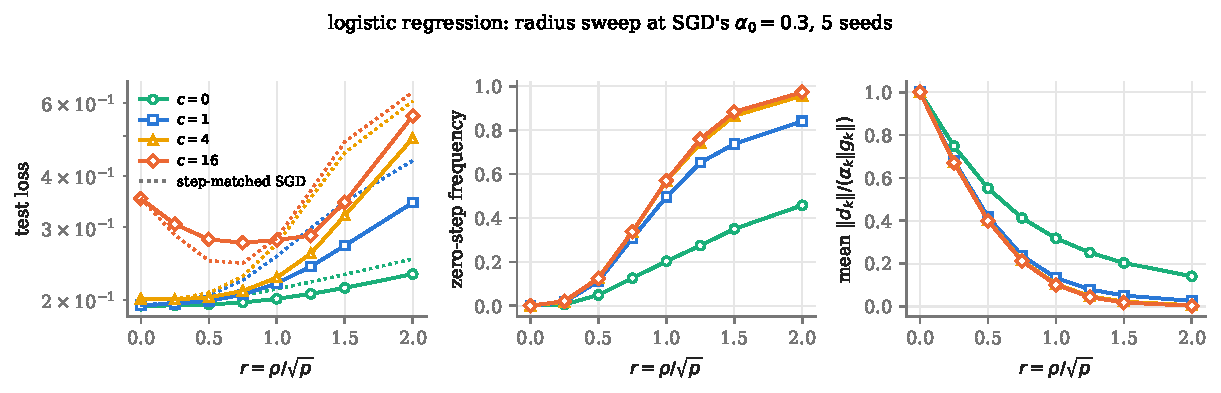
\includegraphics[width=\linewidth]{../fig3/logreg_sensitivity.pdf}
\caption{Логистическая регрессия, перебор радиуса при $\alpha_0=0.3$ (настройка SGD), 5 сидов.
Слева: потери на тесте R-SGD (сплошные) и SGD с той же длиной шага (пунктир). В центре: доля
нулевых шагов. Справа: среднее отношение $\|d_k\|/(\alpha_k\|g_k\|)$.}
\label{fig:lr_sens}
\end{figure}

\begin{center}
\small
\setlength{\tabcolsep}{4pt}
\begin{tabular}{@{}ccccccccc@{}}
\toprule
$c$ & $r$ & \shortstack{нулевые\\шаги} & \shortstack{отн.\\шага} & \shortstack{потери\\обуч.} & \shortstack{потери\\тест} & \shortstack{контр.\ SGD\\тест} & \shortstack{побед\\R} & точность \\
\midrule
\tabinput{../tabs3/tab_lr_sens.tex}
\bottomrule
\end{tabular}

\smallskip
Логистическая регрессия, перебор радиуса при $\alpha_0=0.3$ (средние по 5 сидам); $r=0$ — SGD.
\end{center}

\begin{itemize}
\item При $c\le4$ рост $r$ не снижает потери (не более чем на $0.0007$ при $r=0.25$, затем они
растут): при настроенном шаге SGD выигрывать нечего. Но R-SGD лучше SGD с той же средней длиной
шага при каждом $r$ в 5/5 сидов (один раз 4/5). Его сжатие мало в начале (большие градиенты,
высокое отношение сигнал/шум) и велико в конце, то есть работает как адаптивное уменьшение шага;
постоянное уменьшение теряет скорость в начале.
\item При $c=16$ значения $r=0.5$--$0.75$ снижают потери на тесте с $0.352$ до $0.275$, но
контрольный SGD даёт лучше ($0.246$, R-SGD выигрывает в 1/5): выигрыш — эффект длины шага.
\item Точность почти не меняется с $r$ (в пределах $0.002$ при $c\le4$), пока не начинают
доминировать нулевые шаги.
\end{itemize}

\begin{center}
\small
\begin{tabular}{@{}ccccccccc@{}}
\toprule
& \multicolumn{4}{c}{sd потерь на тесте} & \multicolumn{4}{c}{sd точности на тесте} \\
\cmidrule(lr){2-5}\cmidrule(lr){6-9}
$c$ & SGD A & SGD B & R-SGD A & R-SGD B & SGD A & SGD B & R-SGD A & R-SGD B \\
\midrule
\tabinput{../tabs3/tab_lr_var.tex}
\bottomrule
\end{tabular}

\smallskip
Логистическая регрессия: разброс по наборам данных и случайности обучения (A) против разброса
только по случайности обучения (B).
\end{center}
При $c\le1$ доминирует разброс по наборам данных (sd в A в 2--7 раз больше, чем в B); при $c\ge4$
главным источником становится случайность обучения из-за добавленного шума.

\section*{Шаг 3. Эксперимент 2: двухслойная сеть}

\subsection*{3.1 Модель, инициализация, градиент}

Полуокружности: $t\sim U[0,\pi]$, класс 0 в точке $(\cos t,\sin t)+e$, класс 1 в точке
$(1-\cos t,\tfrac12-\sin t)+e$, $e\sim\mathcal N(0,0.1^2I_2)$. Модель
$t_\theta(a)=w_2^T\tanh(W_1a+b_1)+b_2$ с 8 скрытыми нейронами, $p=33$. Инициализация:
$W_1\sim\mathcal N(0,\tfrac12)$, $b_1=0$, $w_2\sim\mathcal N(0,\tfrac18)$, $b_2=0$ (дисперсия
$1/\text{fan-in}$), из потока инициализации данного сида; SGD и R-SGD стартуют из одной и той же
$\theta_0$. Начальные потери близки к $\log2=0.693$. Градиент вычисляется обратным
распространением по каждому примеру (раздел 2, шаг 3); проверка конечными разностями в
фактической начальной точке даёт относительные ошибки $4.9\cdot10^{-10}$ (средний) и
$8.9\cdot10^{-10}$ (по примерам).

\subsection*{3.2 Настройка}

Выбрано (рис.~\ref{fig:tuning}, справа): SGD $\alpha_0=1$; R-SGD $\alpha_0=10$, $r=0.25$
($\rho=1.44$). Ни одна настройка не на краю. Критерий R-SGD ($0.0104$) меньше, чем у SGD
($0.0138$), но поверхность нерегулярна: $(10,0)$, то есть SGD с $\alpha_0=10$, даёт $0.0156$,
$(10,0.5)$ — $0.0184$, $(10,0.75)$ — $0.0117$. Такие немонотонные соседи показывают, что разности
этого масштаба лежат в пределах шума оценки по 3 сидам. Последствия видны в п.~3.3.

\subsection*{3.3 Результаты}

\begin{figure}[H]
\centering
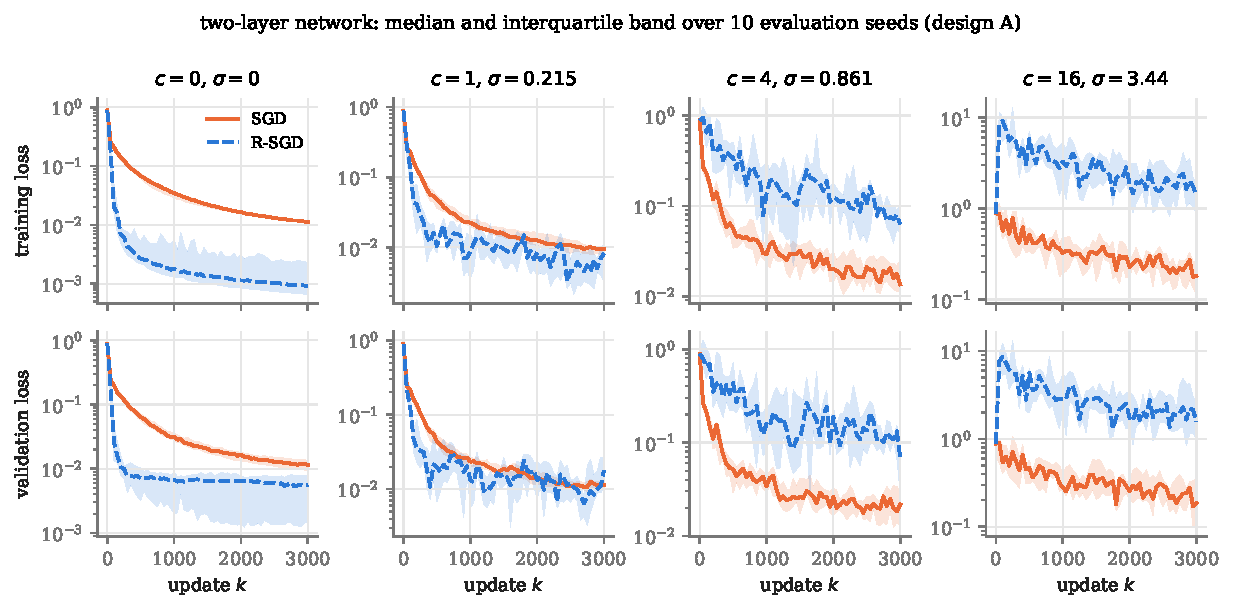
\includegraphics[width=\linewidth]{../fig3/mlp_curves.pdf}
\caption{Двухслойная сеть: потери на обучении (сверху) и на валидации (снизу) на чистых
данных, медиана и интерквартильная полоса по 10 сидам оценки (схема A). Зафиксированные
настройки: SGD $\alpha_0=1$; R-SGD $\alpha_0=10$, $\rho=1.44$.}
\label{fig:mlp_curves}
\end{figure}

\begin{center}
\small
\setlength{\tabcolsep}{4pt}
\begin{tabular}{@{}clccccc@{}}
\toprule
$c$ & метод & \shortstack{итог.\ потери\\обуч.} & \shortstack{потери\\на тесте} & \shortstack{точность\\на тесте} & \shortstack{нулевые\\шаги} & \shortstack{время, мс\\(мкс/обн.)} \\
\midrule
\tabinput{../tabs3/tab_mlp_main.tex}
\bottomrule
\end{tabular}

\smallskip
Двухслойная сеть, схема A, среднее $\pm$ sd по 10 сидам; $bK=48\,000$ вычислений градиента за
запуск у обоих методов.
\end{center}

\begin{center}
\footnotesize
\setlength{\tabcolsep}{2.6pt}
\begin{tabular}{@{}cccccccccc@{}}
\toprule
& & \multicolumn{2}{c}{$\Delta$ потерь обуч.} & \multicolumn{2}{c}{$\Delta$ потерь на тесте}
& \multicolumn{2}{c}{$\Delta$ точности} & \multicolumn{2}{c}{совпадение} \\
\cmidrule(lr){3-4}\cmidrule(lr){5-6}\cmidrule(lr){7-8}\cmidrule(lr){9-10}
$c$ & схема & среднее $\pm$ h & побед & среднее $\pm$ h & побед & среднее $\pm$ h & \shortstack{побед\\(ничьи)} & \shortstack{об.$\to$\\тест} & \shortstack{об.$\to$\\точн.} \\
\midrule
\tabinput{../tabs3/tab_mlp_paired.tex}
\bottomrule
\end{tabular}

\smallskip
Двухслойная сеть: парные разности R-SGD $-$ SGD, как в таблице для логистической регрессии.
\end{center}

Как читать результаты.
\begin{itemize}
\item \textbf{$c=0$: R-SGD оптимизирует быстрее.} Потери на обучении $0.0019$ против
$0.0110$ (10/10 сидов в обеих схемах); потери на тесте меньше в 9/10 (A) и 10/10 (B). Кривые на
рис.~\ref{fig:mlp_curves} расходятся через несколько сотен обновлений. Точность не лучше
(3 победы, 2 ничьи), так как оба метода уже правильно классифицируют $99.8\%$ тестовых точек.
\item \textbf{Выигрыш при $c=0$ — выигрыш длины шага.} Среднее отношение шагов R-SGD $0.59$,
поэтому он движется как SGD с $\alpha_0'=5.9$, в шесть раз большим настроенного для SGD $1$. Такой
SGD достигает потерь на тесте $0.0065$ против $0.0082$ у R-SGD (R-SGD лучше в 4/10). Значение
$\alpha_0=1$ для SGD выбрано при $c=1$ по шумному критерию, а не при $c=0$.
\item \textbf{$c=1$, сам уровень настройки: R-SGD хуже.} Потери на валидации при оценке
$0.0230\pm0.0207$ против $0.0114\pm0.0028$ у SGD, хотя настройка предсказывала обратное
($0.0104$ против $0.0138$). Выбор R-SGD — минимум по 36 шумным оценкам против 6 у SGD, поэтому он
смещён в оптимистичную сторону («проклятие победителя»), а выбранный большой $\alpha_0=10$ —
настройка с большой дисперсией. Точность на тесте $0.9946$ против $0.9980$; SGD лучше в 8 из 10
сидов (одна ничья).
\item \textbf{$c\ge4$: зафиксированная настройка R-SGD разваливается.} Потери на тесте $0.115$
против $0.025$ ($c=4$) и $1.96$ против $0.22$ ($c=16$); при $c=16$ 8 из 10 запусков R-SGD
заканчиваются потерями на обучении выше начальных $\log2$. Эффективный шаг около
$7.4/\sqrt{1+k/50}$, то есть в 7.4 раза больше, чем у SGD, при градиентах, в которых доминирует
шум, выбрасывает сеть в области насыщения. Ни один запуск не попал под формальный критерий
неудачи (потери $>50$ начальных).
\item \textbf{Нулевые шаги:} при выбранном $\rho=1.44$ их нет: это намного меньше порога для
режима доминирующего шума $\approx\sqrt{p(b-1)/(b-3)}=6.2$.
\item \textbf{Время:} SGD 32--49\,мкс на обновление, R-SGD 109--128\,мкс (в 2.6--3.6 раза
больше).
\end{itemize}

\begin{figure}[H]
\centering
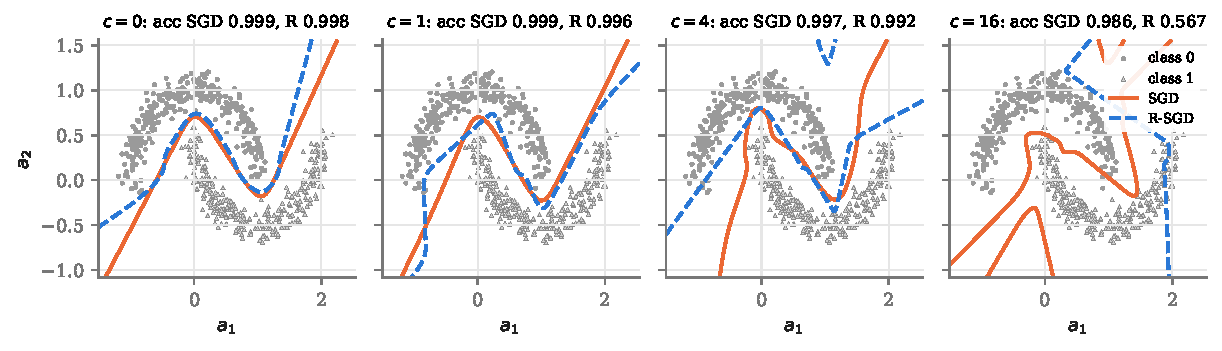
\includegraphics[width=\linewidth]{../fig3/mlp_boundaries.pdf}
\caption{Двухслойная сеть, сид оценки A-0: границы решения итоговых точек SGD и R-SGD в
исходных координатах и 600 тестовых точек. Вдали от данных границы экстраполируют по-разному,
даже когда обе разделяют полуокружности (две левые панели).}
\label{fig:mlp_bound}
\end{figure}

\subsection*{3.4 Длина шага, чувствительность и разброс}

\begin{center}
\small
\setlength{\tabcolsep}{4pt}
\begin{tabular}{@{}cccccccc@{}}
\toprule
$c$ & \shortstack{отн.\\шага} & $\alpha_0'$ & потери R-SGD & \shortstack{потери SGD\\с той же длиной} & $\Delta$ (R $-$ контр.) & побед & \shortstack{точн.\\R / контр.} \\
\midrule
\tabinput{../tabs3/tab_mlp_matched.tex}
\bottomrule
\end{tabular}

\smallskip
Двухслойная сеть: зафиксированный R-SGD против SGD с той же средней длиной шага, схема A,
10 сидов.
\end{center}

\begin{figure}[H]
\centering
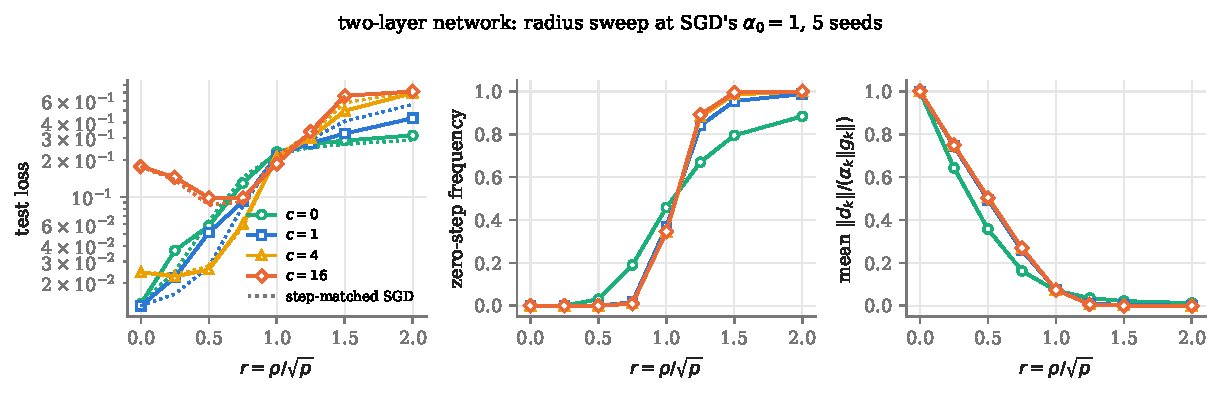
\includegraphics[width=\linewidth]{../fig3/mlp_sensitivity.pdf}
\caption{Двухслойная сеть, перебор радиуса при $\alpha_0=1$ (настройка SGD), 5 сидов. Слева:
потери на тесте R-SGD (сплошные) и SGD с той же длиной шага (пунктир). В центре: доля нулевых
шагов. Справа: среднее отношение шагов.}
\label{fig:mlp_sens}
\end{figure}

\begin{center}
\small
\setlength{\tabcolsep}{4pt}
\begin{tabular}{@{}ccccccccc@{}}
\toprule
$c$ & $r$ & \shortstack{нулевые\\шаги} & \shortstack{отн.\\шага} & \shortstack{потери\\обуч.} & \shortstack{потери\\тест} & \shortstack{контр.\ SGD\\тест} & \shortstack{побед\\R} & точность \\
\midrule
\tabinput{../tabs3/tab_mlp_sens.tex}
\bottomrule
\end{tabular}

\smallskip
Двухслойная сеть, перебор радиуса при $\alpha_0=1$ (средние по 5 сидам); $r=0$ — SGD.
\end{center}

\begin{itemize}
\item При $c\le1$ любое $r>0$ ухудшает результат; при $c=4$ эффект $r\le0.5$ в пределах шума.
\item При $c=16$ значения $r=0.5$--$0.75$ улучшают потери на тесте с $0.176$ до $0.098$ и
точность с $0.953$ до $0.968$, но контрольный SGD ещё лучше ($0.086$; R-SGD выигрывает 2/5 и
1/5). В режиме доминирующего шума робастный шаг ведёт себя как укороченный шаг SGD.
\item \textbf{Нулевые шаги до минимума.} При $r\ge1$ доля нулевых шагов скачком растёт до
35--100\%, и обучение останавливается при точности $0.91$--$0.50$. При $c=4,16$ и $r=2$ сеть
практически не движется (99.9--100\% нулевых шагов, точность $0.50$). Объяснение (шаг 4): когда
доминирует шум, $g_k^TS_k^{-1}g_k$ близко к своему значению в стационарной точке независимо от
$\theta_k$, поэтому проверка нулевого шага не может определить, близка ли итерация к минимуму.
\end{itemize}

\begin{center}
\small
\begin{tabular}{@{}ccccccccc@{}}
\toprule
& \multicolumn{4}{c}{sd потерь на тесте} & \multicolumn{4}{c}{sd точности на тесте} \\
\cmidrule(lr){2-5}\cmidrule(lr){6-9}
$c$ & SGD A & SGD B & R-SGD A & R-SGD B & SGD A & SGD B & R-SGD A & R-SGD B \\
\midrule
\tabinput{../tabs3/tab_mlp_var.tex}
\bottomrule
\end{tabular}

\smallskip
Двухслойная сеть: разброс по наборам данных и случайности обучения (A) против разброса только
по случайности обучения (B).
\end{center}
Для сети разброс в B (случайность обучения, включая инициализацию) сравним с разбросом в A, в
отличие от логистической регрессии: невыпуклая модель чувствительна к инициализации и к
траектории. При 10 сидах сама оценка sd неопределённа примерно на $\pm25\%$, поэтому значимы
только большие отношения.

\section*{Шаг 4. Почему R-SGD ведёт себя именно так}

\textbf{Режим доминирующего шума.} Пусть добавленный шум доминирует в покоординатной дисперсии
наблюдений. Тогда все $\widehat s_{k,j}$ близки к $\sigma^2/b$ (с точностью до флуктуаций
$\chi^2_{b-1}$), так что $S_k\approx sI$ с $s\approx\sigma^2/b$, и работает изотропная формула
из 1(d):
\begin{equation*}
d_k\approx-\alpha_k\Big(1-\frac{\rho\sqrt s}{\norm{g_k}}\Big)_+g_k,\qquad
\norm{d_k}=\alpha_k\big(\norm{g_k}-\rho\sqrt s\big)_+ .
\end{equation*}
Направление совпадает с направлением SGD; меняется только длина. Поскольку $g_k$ в основном
шум, $\norm{g_k}^2\approx\sum_j\Var(g_{k,j})\approx ps$, и при $\rho=r\sqrt p$
\begin{equation*}
\frac{\norm{d_k}}{\alpha_k\norm{g_k}}\approx1-\frac{r\sqrt p\,\sqrt s}{\sqrt{ps}}=1-r .
\end{equation*}
Измерено для сети при $c\ge4$: $0.748,\,0.505,\,0.269$ при $r=0.25,0.5,0.75$; предсказание
$0.75,\,0.50,\,0.25$. При $p=3$ согласие грубее ($0.67,0.40,0.21$), потому что в трёх измерениях
$\norm{g_k}$ флуктуирует сильнее. Следствия:
\begin{itemize}
\item В этом режиме R-SGD в первом приближении — это SGD с шагом $\alpha_k(1-r)$. Он не может
быть лучше SGD, длина шага которого настроена при том же уровне шума, что и показывают
контрольные запуски.
\item Во втором приближении он хуже постоянного уменьшения шага: множитель
$1-\rho\sqrt s/\norm{g_k}$ \emph{растёт} с $\norm{g_k}$, поэтому самые большие (самые шумные)
реализации сжимаются меньше всего. Робастный шаг выполняет мягкое пороговое отсечение нормы
градиента, а не уменьшение дисперсии.
\item С настройками, зафиксированными при $c=1$, R-SGD перенёс большой $\alpha_0$ (в 3 и 10 раз
больше, чем у SGD) на более сильный шум, где сжатие уже не компенсирует его нужным образом.
\end{itemize}

\textbf{Порог нулевого шага при шуме.} При $c\ge1$ каждое $g_{k,j}/\sqrt{\widehat s_{k,j}}$
приближённо имеет распределение Стьюдента с $b-1$ степенями свободы при любом $\theta_k$, так что
$g_k^TS_k^{-1}g_k\approx\sum_jt_j^2$ со средним $p(b-1)/(b-3)$. Тогда вероятность нулевого шага
почти полностью определяется $r$: он редок при $r<1$ и почти неизбежен при
$r>\sqrt{(b-1)/(b-3)}=1.07$. Это объясняет резкие скачки между $r=1$ и $r=1.5$ на
рис.~\ref{fig:lr_sens} и \ref{fig:mlp_sens} и «замёрзшую» сеть: эти нулевые шаги происходят
далеко от любого минимума.

\textbf{Режим малого шума.} При $c\le1$ дисперсии сильно различаются по координатам и во
времени. Тогда сжатие зависит от отношения сигнал/шум: слабое в начале, сильное вблизи
минимума. В логистической регрессии это адаптивное уменьшение выиграло у любого постоянного
уменьшения с тем же средним (5/5 сидов при всех $r$) — это настоящий, хотя и малый, эффект
робастного шага. Он снижает потери, но не долю ошибок.

\textbf{Невыпуклость.} Робастная подзадача (2) сильно выпукла на каждом шаге, поэтому $d_k$
единственен, а решатель точен (раздел 2). Это ничего не гарантирует для невыпуклой $f$ сети:
шаг робастен только относительно локальной линейной модели. Остановившиеся запуски показывают,
что правило нулевого шага не отличает минимум от точки, где шум скрывает градиент.

\section*{Шаг 5. Совпадают ли ранжирования по оптимизации и по предсказанию?}

\begin{itemize}
\item \textbf{Потери на обучении и на тесте: в основном да.} На фиксированном наборе данных
(схема B) знак $\Delta$ потерь на обучении предсказывал знак $\Delta$ потерь на тесте в 7--10 из
10 сидов во всех случаях, кроме сети при $c=1$ (3/10). В схеме A исключения — сеть при $c=1$
(5/10) и логистическая регрессия при $c=0$ (2/10), где разности $0.002$ тонут в разбросе между
наборами данных. Оба набора данных простые, и при 400 обучающих точках модели далеки от
переобучения.
\item \textbf{Потери на обучении и точность: при малом шуме нет.} Логистическая регрессия при
$c\le1$: совпадение 3--5/10; сеть при $c=0$: 3/10, хотя потери R-SGD на обучении в 5.8 раза
меньше. Меньшая кросс-энтропия здесь в основном означает более уверенные логиты на уже
правильно классифицированных точках. Логистическая регрессия находится на байесовской
точности, поэтому никакой оптимизатор не может её повысить; в сети оба метода на уровне $99.8\%$.
\item \textbf{При большом шуме все ранжирования совпадают} (7--10/10): шум портит саму границу, и
метод с меньшими потерями и классифицирует лучше.
\item Для обоих экспериментов вместе: меньшие потери на обучении, меньшие потери на тесте и
более высокая точность — разные результаты, как и сказано в критерии успеха задания. В этих
экспериментах R-SGD иногда добивался первых двух; более высокой точности, чем у SGD с той же
средней длиной шага, он не добился ни разу.
\end{itemize}

\section*{Шаг 6. Воспроизводимость}

\begin{itemize}
\item \textbf{Код.} \texttt{sim3\_core.py} (данные, стандартизация, цикл обучения с чистой
оценкой и замером времени), \texttt{sim\_section3.py} (настройка, оценка, перебор, контроль,
рисунки), \texttt{make\_tables3.py} (все таблицы отчёта), \texttt{rsgd.py} из раздела 2. Команды:
\texttt{python sim\_section3.py run} (около 3 минут, пишет \texttt{results\_section3.json} и
\texttt{curves\_section3.npz}), затем \texttt{python make\_tables3.py}.
\item \textbf{Сиды.} Главный сид $20261118$. У каждого сида четыре независимых потока (данные,
инициализация, индексы батчей, шум градиента) из
\texttt{SeedSequence([20261118, sim, kind, seed])}, где sim $=1$ (логистическая) или $2$ (сеть),
kind $=0$ (сиды настройки 0--2), $1$ (сиды схемы A 0--9), $2$ (сиды схемы B 0--9; их поток данных
заменён потоком A-сида 0). Границы решения построены для A-сида 0.
\item \textbf{Общие случайные числа.} SGD и R-SGD для каждого сида используют одинаковые потоки.
\item \textbf{Замер времени.} Замеряются только $K$ обновлений (выбор батча, градиенты, шум,
$g_k$, $S_k$, шаг); контрольные точки оценки исключены. Python 3.13, NumPy 2.5.3, одно ядро.
\item \textbf{Неудачные запуски.} По указанному критерию их нет ни в настройке, ни в оценке, ни
в переборе; 8 запусков сети с итоговыми потерями выше $\log2$ при $c=16$ описаны выше.
\end{itemize}

\section*{Замечания для разделов 4--5}

\begin{itemize}
\item \textbf{Шум настройки.} Трёх сидов настройки для сети не хватило: выбор для R-SGD не
воспроизвёлся даже на его собственном уровне шума. Больше сидов или правило, предпочитающее
плоские области критерия, сделали бы сравнение надёжнее. Больший бюджет поиска R-SGD (108 против
18 запусков) даёт ему преимущество при выборе, и его нужно указывать рядом с любым выигрышем.
\item \textbf{Фиксация при $c=1$} требуется протоколом, но она определяет исход при $c\ge4$.
Сфокусированный следующий эксперимент: настроить оба метода отдельно на каждом уровне шума и
сравнить R-SGD с SGD, настроенным с тем же бюджетом.
\item \textbf{Диагональная $S_k$.} Она игнорирует корреляции между 33 параметрами сети; в
режиме доминирующего шума это не важно, так как добавленный шум изотропен.
\end{itemize}

\end{document}
